%Correct the file name.
%X: book number
%Y: part number
%ZZZ: page number in three digits. So page 3 would be 003.

\documentclass[11pt]{amsbook}

\usepackage{../HBSuerDemir}	
\begin{document}

% ++++++++++++++++++++++++++++++++++++++
\hPage{b1p2/271}
% ++++++++++++++++++++++++++++++++++++++

\begin{exmp}
	 Given the points $A(t, 3)$, $B(4, 5)$ and $C(4.8)$ 
	\begin{hEnumerateAlpha}
		\item Find t if $A$, $B$, $C$ are collinear (Points of the same line) 

		\item Setting $t=-2$ find the equations of the lines $AB$ and $BC$. 

		\item Find the equation of the line through B and P(l, -1) 

		\item $d(P, BC)$, $d(P, AB)$ 
	\end{hEnumerateAlpha}

	\begin{hSolution}
		\begin{hEnumerateAlpha}
			\item Setting the coordinates of point in $Ax + By + C = 0$  we have the HLS 
			$$tA + 3B + C = 0$$ $$4A + 5B + C = 0$$ $$4A + 8B + C = 0$$ 
			To have a non trivial solution we get
		%\[
		 \begin{align*}
			\begin{vmatrix}
			t & 3 & 1 \\ 
			4 & 5 & 1 \\
			4 & 8 & 1 
			\end{vmatrix}
			=0   
			\hspace{1cm}  \text{giving  $t = 4$.} 
		\end{align*}
	
		%\] 
   
   	       This is one of the ways of solution. The others are:
	       \begin{hEnumerateArabic}
			\item  By the use of distance: For the collinearity, one of $\mid AB \mid$,$\mid BC \mid$ and $\mid CA \mid$ must be the sum of the 				other two.
			\item By the use of slope: For the collinearity. the slopes of $AB$ and $BC$ must be equal. 
			\item By the use of equation: For the collinearity, the coordinate of one of the points, say of $A$, must satisfy the equation of the line 					through the other two points $B$, $C$. (This mean that $d(A, BC) = 0$ )
		\end{hEnumerateArabic}
	
		 \item \( \frac{x - x_1}{x_2 - x_1} \) \( \frac{y - y_1}{y_2 - y_1} \) $\Rightarrow$ \\
   		  
		  $AB$: \( \frac{x + 2}{y + 2} \) \( \frac{y - 3}{y - 3} \) $\Rightarrow$ $x - 3y + 11 = 0$, \\	
   
       		  $BC$: $x_1 = x_2 = 4$ $\Rightarrow$ $x = 4$
		
		\end{hEnumerateAlpha}
	\end{hSolution}
\end{exmp}
%==== templates ====

%==== environments ====

%\begin{figure}[htb]
%	\centering
%	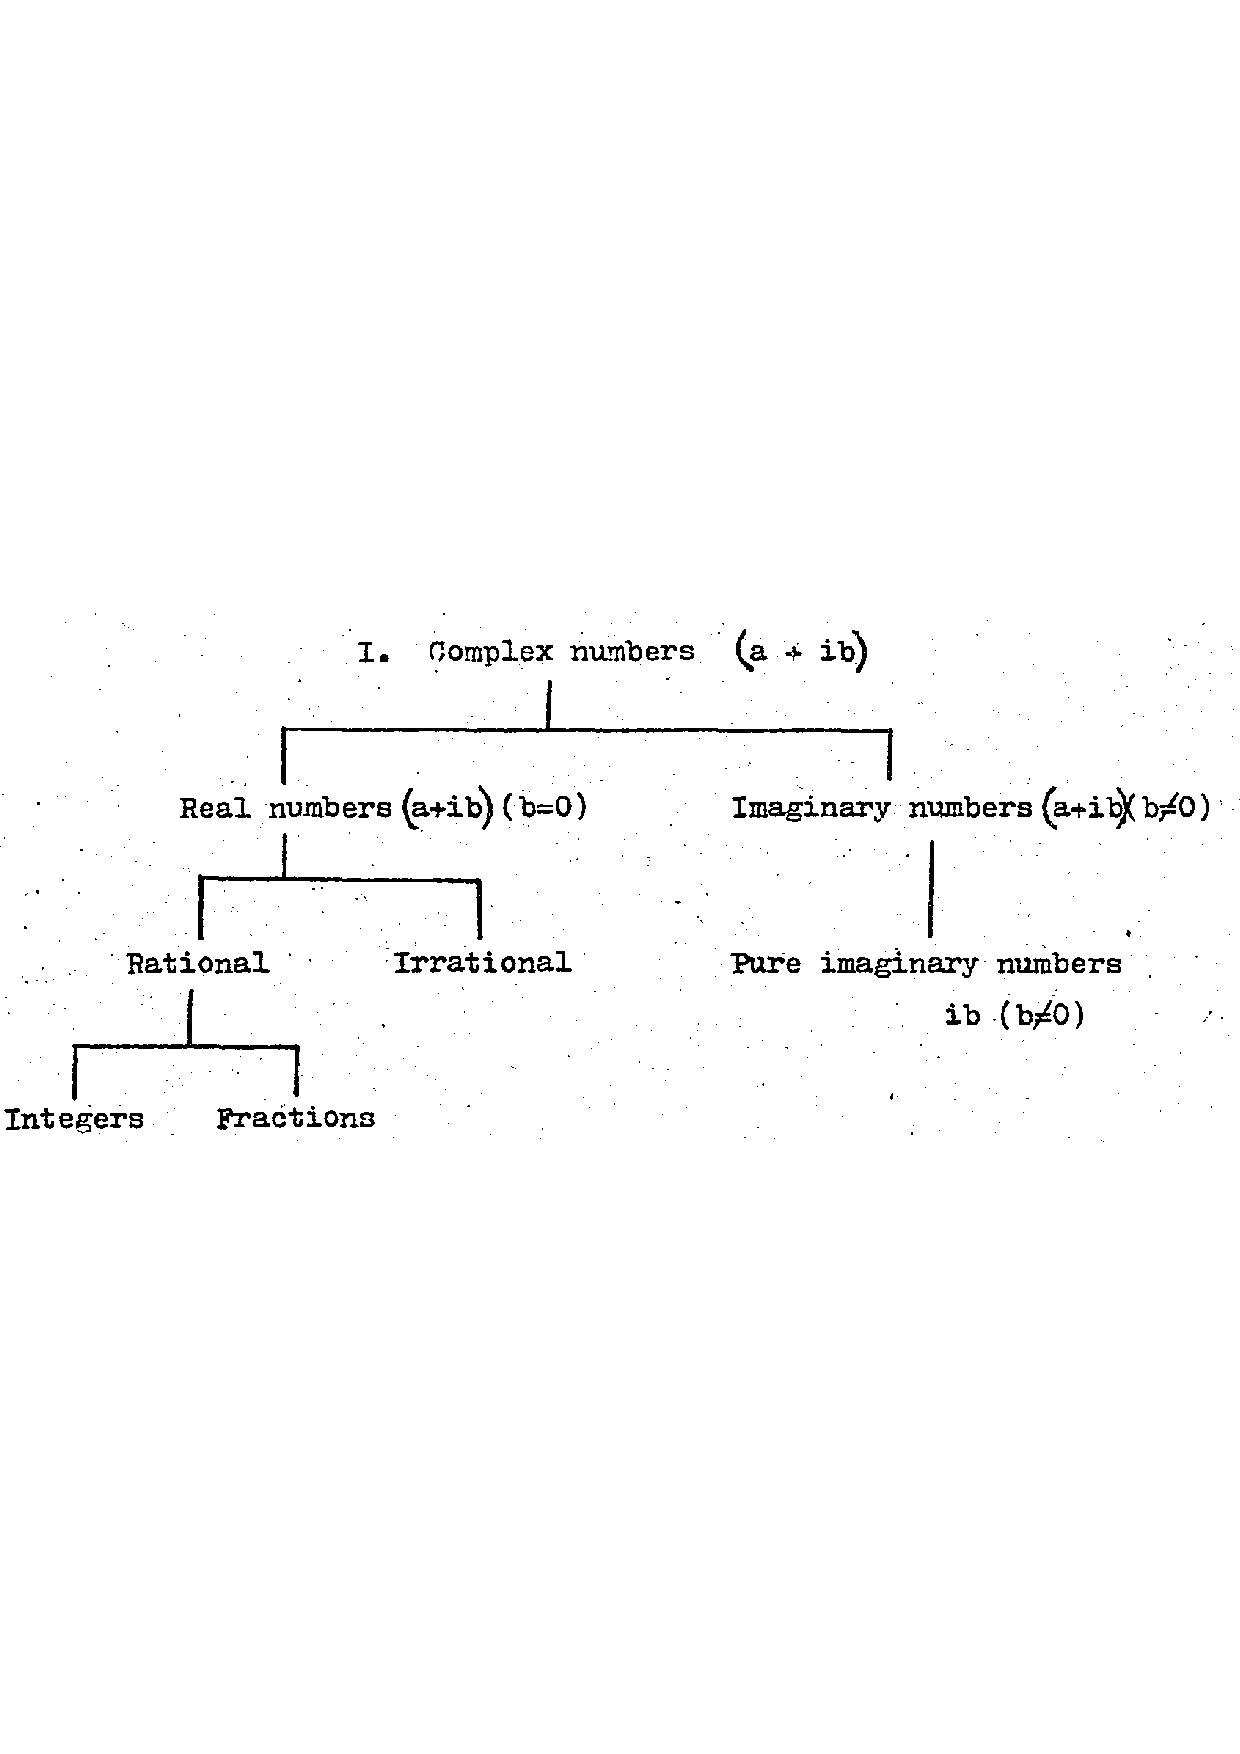
\includegraphics[width=0.9\textwidth]{images/SD-1-1p15A}
%	\caption{Classification of complex numbers}
%	\label{fig:classificationOfComplexNumbersA}
%\end{figure}

%\begin{center}
%\begin{tabular}{cc}
%\end{tabular}
%\end{center}

%\begin{exmp}
%\begin{hSolution}
%\end{hSolution}
%\end{exmp}

%\begin{hEnumerateAlpha}
%\end{hEnumerateAlpha}

%\begin{hEnumerateRoman}
%\end{hEnumerateRoman}

%$
%\begin{bmatrix}
%\end{bmatrix}
%$

%\frac{aaaa}{bbb}
%\frac{a_{n}}{b_{n}}
%\left( aaaa \right)
%\Longrightarrow

%\begin{multicols}{2}
%	bb
%\columnbreak
%	aa
%\end{multicols}

\end{document}  


